\newpage
\let\cleardoublepage\clearpage
\part{Информационно-коммуникационные и химические технологии}
\chapter{Информационно-коммуникационные технологии}
{МРНТИ 20.23.17}
\hfill {\bfseries \href{https://doi.org/10.58805/kazutb.v.3.24-495}{https://doi.org/10.58805/kazutb.v.3.24-495}}


\sectionwithauthors{Д.К. Даркенбаев,Г.З.Зиятбекова, А. Алтыбай, Н.О. Мекебаев,Д.С.Жамангарин}{ИССЛЕДОВАНИЕ СИСТЕМ КРЕДИТНОГО СКОРИНГА С ИСПОЛЬЗОВАНИЕМ
АЛГОРИТМОВ МАШИННОГО ОБУЧЕНИЯ}

\begin{center}
{\bfseries \textsuperscript{1}Д.К. Даркенбаев, \textsuperscript{1}Г.З.
Зиятбекова\envelope, \textsuperscript{1}А. Алтыбай,
\textsuperscript{2}Н.О. Мекебаев, \textsuperscript{3}Д.С.Жамангарин}

\textsuperscript{1}Казахский национальный университет имени аль-Фараби,
Алматы, Казахстан,

\textsuperscript{2}Казахский национальный женский педагогический
университет, Алматы, Казахстан,

\textsuperscript{3}Казахский университет технологии и бизнеса им.К.Кулажанова, Астана,
Казахстан
\end{center}
\envelope Корреспондент-автор: ziyatbekova@mail.ru \vspace{0.5cm}

В статье использовались алгоритмы машинного обучения для решения задач
кредитного скоринга. Изучены методы анализа, прогнозирования и
определения платежеспособности физических лиц. Кроме того, в статье
сравнивается и исследуется одна из актуальных проблем банковских систем,
а также представлены результаты обработки данных. Результаты
исследования, представленные в статье, показали эффективность кредитного
скоринга при принятии решений и показали, что их использование позволяет
существенно повысить точность прогнозирования кредитоспособности
фи-зических лиц и улучшить процесс принятия решений по кредитованию.
Результаты исследования, представленные в статье, вносят важный вклад в
банковскую отрасль и решают проблемы принятия решений по финансированию
физических лиц. Практическое применение результатов поможет улуч-шить
процесс кредитования и снизить риски финансовых организаций. Авторы
статьи планируют продолжить исследования в этой области.

{\bfseries Ключевые слова:} методы, технология, данные, алгоритм, анализ.


\sectionheading{МАШИНАЛЫҚ ОҚЫТУ АЛГОРИТМДЕРІН ҚОЛДАНАТЫН НЕСИЕЛІК СКОРИНГ
ЖҮЙЕЛЕРІН ЗЕРТТЕУ}
\begin{center}
{\bfseries \textsuperscript{1}Д.К. Даркенбаев, \textsuperscript{1}Г.З.
Зиятбекова\envelope, \textsuperscript{1}А. Алтыбай,
\textsuperscript{2}Н.О. Мекебаев, \textsuperscript{3}Д. С. Жамангарин}

\textsuperscript{1}әл-Фараби атындағы Қазақ ұлттық университеті, Алматы,
Қазақстан,

\textsuperscript{2}Қазақ ұлттық қыздар педагогикалық университеті,
Алматы, Қазақстан,

\textsuperscript{3}Қ. Құлажанов атындағы Қазақ технология және бизнес
университеті, Астана, Қазақстан,

е-mail: ziyatbekova@mail.ru
\end{center}


Мақалада несиелік скоринг мәселелерін шешуде машиналық оқыту
алгоритмдері қолданылды. Жеке тұлғалардың төлем қабілеттілігін талдау,
болжау және анықтау әдістері зерттелген. Сонымен қатар, мақалада банк
жүйелерінің өзекті мәселелерінің бірі несиелік скоринг жүйелері
салыстырыла зерттеліп, деректерді өңдеу нәтижелері берілген. Мақаладағы
берілген зерттеу нәтижелерi несиелік скорингтің шешім қабылдауда
тиiмдiлiгiн көрсетті және оларды қолдану жеке тұлғалардың несие
қабiлеттiлiгiн болжау дәлдiгiн айтарлықтай жақсартуға және несие беру
бойынша шешiм қабылдау процесiн жақсартуға болатындығын көрсетті.
Мақалада берілген зерттеу нәтижелері банк саласына маңызды үлес қосады
және жеке тұлғаларды қаржыландыру бойынша шешім қабылдау мәселелерін
шешеді. Нәтижелердi практикалық қолдану несие беру процесiн жақсартуға
және қаржы ұйымдары-на тәуекелдердi азайтуға септігін тигізеді. Мақала
авторлары осы салада зерттеу жұмыстарын әрі қарай жалғастыруды жоспарлап
отыр.

{\bfseries Түйін сөздер:} әдістер, технология, деректер, алгоритм, талдау.


\sectionheading{RESEARCH OF CREDIT SCORING SYSTEMS USING MACHINE LEARNING
ALGORITHMS}
\begin{center}
{\bfseries \textsuperscript{1}D.K. Darkenbayev,}
{\bfseries \textsuperscript{1}G.Z. Ziyatbekova\envelope,}
{\bfseries \textsuperscript{1}A. Altybay, \textsuperscript{2}N.O.
Mekebayev,} {\bfseries \textsuperscript{3}D.S. Zhamangarin,}

\textsuperscript{1}Al-Farabi Kazakh National University, Almaty,
Kazakhstan,

\textsuperscript{2} Kazakh National Women\textquotesingle s Pedagogical
University, Almaty, Kazakhstan,

\textsuperscript{3}K. Kulazhanov Kazakh University of Technology and
Business, Astana, Kazakhstan,

е-mail: ziyatbekova@mail.ru
\end{center}


The article used machine learning algorithms to solve credit scoring
problems. Methods of analysis, forecasting and determination of the
solvency of individuals have been studied. In addition, the article
compares and examines one of the current problems of banking systems,
and also presents the results of data processing. The research results
presented in the article showed the effectiveness of credit scoring in
decision making and showed that their use can significantly increase the
accuracy of forecasting the creditworthiness of individuals and improve
the lending decision-making process. The research results presented in
the article make an important contribution to the banking industry and
solve the problems of decision-making on financing of individuals.
Practical application of the results will help improve the lending
process and reduce the risks of financial organizations. The authors of
the article plan to continue research in this area.

{\bfseries Keywords:} methods, technology, data, algorithm, analysis.


\begin{multicols}{2}

{\bfseries Введение}. Кредитный скоринг играет важную роль в современном
финансовом секторе Казахстана. Встроенная в процесс принятия кредитных
решений, она позволяет банкам и финансовым учреждениям оценивать
кредитоспособность заемщиков на основе различных факторов, таких как
история платежей, уровень дохода и кредитная история. Это снижает риски
невозврата и невыплаты кредитов, повышает эффективность кредитного
процесса, повышает финансовую устойчивость отрасли. Кредит -- довольно
распространенный термин среди жителей страны {[}1{]}. Изначально
кредитными услугами воспользовались казахстанцы, занимающиеся
предпринимательством или желающие приобрес-ти транспортные средства. Но с
появлением филиалов иностранных банков, таких как Freedom Finance Bank,
Home Credit Bank и других, кредитная система начала развиваться и стала
еще доступнее для каждого жителя страны, имеющего счет в банке.
Значимость кредитного скоринга для банковского сектора Казахстана
определяется в снижении кредитных рисков, повышении эффективности банков
и обеспечении финансовой устойчивости сектора. С появлением услуг
микрокредитования, а также кредитов в рассрочку, ипотеки, кредитов банки
стали получать поминутные заявки на кредит, что вначале было выгодно
финансовым учреждениям из-за процентов, которые они могли получить с
каждого клиента, но разнообразия финансовых история каждого клиента,
требовала индивидуального подхода к каждому, что приводило к
непродуктивной работе сотрудников банка, что соответственно снижало
прибыль. Это послужило стимулом для совершенствования и автоматизации
процесса выдачи кредитов, термина «кредитный скоринг» и применения
машинных алгоритмов {[}2{]}. Использование машинных алгоритмов позволяет
банкам более точно оценить кредитоспособность заемщиков, оптимизировать
процесс выдачи кредита и снизить риск для обеих сторон. Проблема, над
которой мы работаем, связана с кредитным скорингом и его улучшением с
помощью алгоритмов машинного обучения. Кредитный скоринг является
неотъемлемой частью кредитного процесса и его целью является оценка
кредитоспособности заемщика. Точность и эффективность кредитного
скоринга имеют решающее значение для банков и других финансовых
учреждений, поскольку они позволяют снизить риск дефолта и принимать
обоснованные решения о кредитовании. Практическая значимость нашей
работы заключается в том, что ее результаты могут быть использованы
финансовыми учреждениями для улучшения процессов принятия кредитных
решений {[}3{]}. Более точные и эффективные модели кредитного скоринга
позволят банкам принимать обоснованные и обоснованные решения о
кредитовании на основе того факта, что мы определяем неспособность
клиента погасить кредиты, тем самым минимизируя финансовый риск. Таким
образом, проблема недостаточной точности и эффективности традиционных
методов кредитного скоринга, а также необходимость применения
современных алгоритмов машинного обучения делают нашу работу актуальной
и имеющей практическое значение для финансовых учреждений.

{\bfseries Материалы и методы.} Одним из ограничений машинного обучения в
кредитном скоринге является возможность предвзятости. Несколько
исследований показали, что модели машинного обучения могут
воспроизводить и усиливать существующие искажения в данных. Например,
исследование Hardt и др. (2016) обнаружили, что модель машинного
обучения, обученная на исторических кредитных данных, воспроизводит и
усиливает расовые предубеждения, присутствующие в данных. Чтобы смягчить
эту проблему, исследователи предложили различные методы, такие как
ограничения справедливости и состязательное обучение. Ларрейн и др.
(2017) использовали алгоритмы машинного обучения для прогнозирования
поведения выплат по кредитам в Чили. Они сравнили производительность
нескольких моделей, включая логистическую регрессию, машины опорных
векторов и деревья решений, и обнаружили, что случайные леса
обеспечивают наибольшую точность {[}4{]}.

Данные предоставлены в свободный доступ Хоум Кредит Банком. Набор данных
содержит личную информацию о заемщике, такую \hspace{0pt}\hspace{0pt}как
пол, возраст, цель кредита, семейное положение и т. д. А также
финансовую информацию, такую
\hspace{0pt}\hspace{0pt}\hspace{0pt}\hspace{0pt}как доход, есть ли у
человека машина, есть ли у него дом и т. д. Кроме того, данные
предоставляют кредитную историю человека, ежемесячные выписки по кредиту
и карте. Объединение данных всех таблиц - первостепенная задача для
создания системы кредитного скоринга. Объединение таблиц между собой -
очень важная задача, поскольку плохое или неудачное объединение данных
может привести к потере ценной информации, что в будущем не позволит
повысить производительность. При объединении таблиц возникает проблема
большой размерности данных. Только в основной таблице application\_train
121 атрибут, за исключением target, но следует также учитывать, что при
объединении таблиц может появиться любое количество атрибутов, например
один атрибут из таблицы или 30 атрибутов из таблицы, поэтому после
объединения всех имеющихся данных количество атрибутов может значительно
увеличиться. Подход к решению этой проблемы заключается в обеспечении
устойчивости алгоритмов машинного обучения к бесполезным функциям. Идея
в том, что модель в ходе обучения сама определит важные для нее и
неважные функции.

{\bfseries Логистическая регрессия.} Логистическая регрессия -- это
контролируемый метод машинного обучения и тип множественной регрессии,
который можно использовать для оценки вероятности того, что событие
произойдет для конкретного субъекта (больной/\\здоровый, погашение
кредита/дефолт и т. д.). В задаче классификации логистическая регрессия
называется бинарной, как следует из названия. Она применяется, когда
зависимая переменная является двоичной, что означает, что она может
принимать только два значения, например «да» или «нет», «истина» или
«ложь», «1» или «0» и так далее. Суть логистической регрессии состоит в
том, что пространство значений независимых переменных
($n$-мерное пространство) можно разделить
некоторой линейной границей на две области, соответствующие классам.

Под некоторой линейной границей понимается линейная комбинация
независимых переменных, называемая гиперплоскостью. В случае двух
измерений это просто прямая линия без кривых. В случае трёх -- это
самолёт и так далее. Чем дальше точка находится от гиперплоскости, тем с
большей вероятностью она принадлежит соответствующему классу предметной
области.

Уравнение, описывающее гиперплоскость:

\begin{equation}
	w^Tx_i+b=0
\end{equation}

\begin{equation}
w_1x_1+w_2x_2+\ldots w_ix_i+b=0
\end{equation}

\begin{equation}
\sum_{i=1}^n w_ix_i+b=0 \ ^{ w \in R^n, b \in R}
\end{equation}


где $w_i$-- коэффициенты, определяющие все
семейство прямых, проходящих через точку $(0,0)$. Соотношение w определяет угол линии
к осям. Ненулевой коэффициент $ b$ позволяет линии не проходить через ноль, другими словами, это смещение.
Наклон к осям не меняется, то есть $ b$ определяет семейство параллельных прямых, $n $ -- количество неизвестных переменных.
Геометрический смысл вектора $(w_i, w_n)$ нормален к гиперплоскости {[}5{]}.

$k$ {\bfseries -Nearest Neighbours (KNN).}
$k$-Nearest Neighbours (KNN) -- это тип
алгоритма машинного обучения, используемый для решения задач
классификации и регрессии. KNN основан на простой идее: объекты одного
класса обычно находятся ближе друг к другу в пространстве признаков. KNN
основан на принципе, где $k$ обозначает
количество «ближайших соседей». Когда новый наблюдаемый случай (или
объект) требует классификации, алгоритм KNN просматривает $k$ ближайших соседей этого объекта из
набора обучающих данных. Затем он присваивает объекту класс, наиболее
распространенный среди этих соседей. Если $k=1$, новый объект присваивается классу его ближайшего соседа. В контексте регрессии KNN присваивает новому
объекту среднее значение $k$ ближайших
соседей. Но раз уж мы решили взять в классификацию KNN, то не будем
особо останавливаться на регрессии. Для определения ближайших соседей
можно использовать различные метрики расстояния:
\end{multicols}

\begin{enumerate}
\def\labelenumi{\arabic{enumi}.}
\item
  Евклидовое расстояние:
\end{enumerate}
\begin{equation}
	d(x,y)=\sqrt{\sum_{i} (x_i-y_i)^2}
\end{equation}

\begin{enumerate}
\def\labelenumi{\arabic{enumi}.}
\setcounter{enumi}{1}
\item
  Расстояние Манхэттена:
\end{enumerate}
\begin{equation}
	d(x,y)=\sum_{i} |x_i - y_i|
\end{equation}

\begin{enumerate}
\def\labelenumi{\arabic{enumi}.}
\setcounter{enumi}{2}
\item
  Расстояние Минковского:
\end{enumerate}

\begin{equation}
	d(x,y)=\Bigg(\sum_{i} \bigg(|x_i - y_i|^p \bigg)\Bigg)^\frac{1}{p}
\end{equation}
\begin{multicols}{2}

где $x $ и $y $ -- два экземпляра, а $x_i$ и $y_i$ -- значения признака $i$ для $x$ и $y$
соответственно, а $p$ -- параметр определяющий степень ближайших соседей.

После расчета расстояний до всех соседей в обучающей выборке KNN
выбирает $k$ соседей, расстояние которых
минимально. Когда выбрано число $k$ и метрика расстояния, KNN классифицирует новые наблюдения на основе того,
какие классы наиболее распространены среди их $k$ ближайших соседей {[}6{]}.

{\bfseries Машины опорных векторов (SVM)}. Машины опорных векторов (SVM) --
это тип алгоритма машинного обучения, который в основном используется
для решения задач классификации, хотя его также можно применять для
регрессии и обнаружения выбросов. Целью SVM является поиск гиперплоскости в многомерном пространстве, которая лучше всего разделяет
два класса данных {[}7{]}.\\ Гиперплоскость -- это линия, которая делит
пространство входных объектов, создавая раздел между классами. SVM
стремится найти оптимальную гиперплоскость, которая эффективно разделяет
точки данных на основе их принадлежности к определенному классу -- это
может быть класс 0 или класс 1. Если мы представим, что это линия в
контексте двумерного пространства, разделяющая наши данные. Например:


\begin{equation}
	B_o+B_1X_1+B_2X_2=0
\end{equation}


где коэффициенты $B_1$ и $B_2$ , определяющие наклон линии и точку
пересечения $B_0$, находятся с помощью алгоритма обучения, а $X_1$ и $X_2$ -- две входные переменные.

Линия гиперплоскости позволяет проводить классификацию. Используя
уравнение линии, мы можем вставить входные значения и определить
положение новой точки относительно линии. У нас будет 4 варианта:

1) Если новая точка находится над линией, уравнение дает значение больше
нуля, и мы можем классифицировать эту точку как принадлежащую первому
классу (класс А).

2) Если новая точка находится ниже линии, уравнение дает значение меньше
нуля, и мы относим точку ко второму классу (классу B).

3) Если новая точка находится близко к линии, уравнение дает значение,
близкое к нулю, и классифицировать точку становится сложнее.

4) Если значение велико, это указывает на большую уверенность модели в
своем прогнозе.

\end{multicols}

\begin{figure}[H]
	\centering
	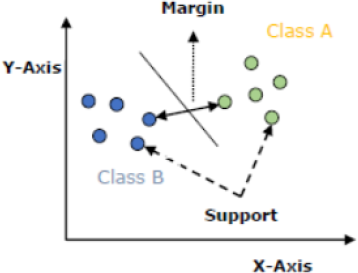
\includegraphics[width=0.5\textwidth]{assets/110}
	\caption*{\bfseries Рис. 1 -- Машины опорных векторов}
\end{figure}


\begin{multicols}{2}

Расстояние между линией и ближайшими точками данных определяется как
«запас». Идеальная или оптимальная линия, которая может эффективно
разделить два класса, имеет наибольший запас. Такая линия называется
«гиперплоскостью с максимальным запасом». Запас определяется как
перпендикулярное расстояние от линии до ближайших точек. Только эти
точки важны при определении линии и создании классификатора. Такие точки
называются «опорными векторами». Они поддерживают или определяют
гиперплоскость. Гиперплоскость выбирается из обучающих данных с
использованием метода оптимизации, который максимизирует запас. На
практике данные часто хаотичны и не могут быть полностью разделены
гиперплоскостью. Из-за этого мы немного ослабляем ограничение на
максимизацию запаса в виде линии, разделяющей классы. Такой
классификатор обычно называют «классификатором с мягкими границами». Это
изменение позволяет некоторым точкам в наборе обучающих данных нарушать
границу разделительной линии {[}8{]}.

{\bfseries Случайный лес (Random Forest).} Случайный лес --- это метод
ансамблевого обучения, который объединяет несколько деревьев решений для
создания более точного и стабильного прогноза. Суть метода заключается в
построении большого количества различных деревьев решений, а затем
усреднении их прогнозов. Каждое дерево строится независимо от других.
При построении каждого дерева используются следующие случайные элементы
{[}9{]}:

1. Начальная загрузка: для построения каждого дерева из исходной выборки
данных с возвратом выбирается подвыборка. Это означает, что некоторые
экземпляры могут появляться в подвыборке более одного раза, а другие
могут вообще не появляться.

2. Подпространство случайных признаков. В каждом узле дерева решений
выборка признаков ограничивается случайным подмножеством признаков при
выборе оптимального признака для разделения.

Однако следует отметить, что при работе со Random Forest нам не нужно
обрабатывать каждое дерево отдельно. Мы просто обучаем модель на данных,
и она автоматически создает и объединяет все деревья.
\end{multicols}

\begin{figure}[H]
	\centering
	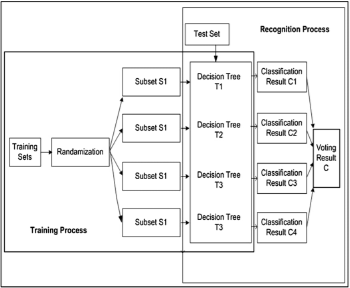
\includegraphics[height=0.45\textwidth, width=0.65\textwidth]{assets/111}
	\caption*{\bfseries Рис. 2 -- Концептуальная основа классификатора случайного леса}
\end{figure}

\begin{multicols}{2}


Существует несколько показателей, которые можно использовать для
измерения «качества» разделения в дереве решений, и эти показатели также
используются в случайном лесу {[}10{]}. Двумя наиболее распространенными
показателями являются энтропия и коэффициент Джини. Обе классификации
являются двоичными и измеряют степень «чистоты» узла.
\end{multicols}

\begin{enumerate}
\def\labelenumi{\arabic{enumi}.}
\item
  Энтропия (в случае бинарной классификации):
\end{enumerate}
\begin{equation}
	E(p)= - p*\log2(p)-(1-p)*\log2(1-p)
\end{equation}

\begin{enumerate}
\def\labelenumi{\arabic{enumi}.}
\setcounter{enumi}{1}
\item
  Коэффициент Джини:
\end{enumerate}

\begin{equation}
	G(p)= 1 - (p^2 + (1 - p)^2)
\end{equation}

\begin{multicols}{2}

где $P$-- вероятность того, что случайно
выбранный элемент из узла будет принадлежать классу 1. Таким образом,
если все элементы в узле принадлежат к одному классу (т.е. узел
«чистый»), энтропия и коэффициент Джини будут равны 0. Если данные
равномерно распределены между обоими классами, они достигнут
максимального значения (в случае бинарной классификации оно будет равно
0,5). В контексте случайного леса энтропия и коэффициент Джини
используются для определения наиболее эффективного разделения на каждом
этапе. Это разделение выбирается таким образом, чтобы минимизировать
взвешенную сумму энтропий или коэффициент Джини в дочерних узлах. Это
помогает создавать деревья решений, которые хорошо распределяют данные,
и приводит к более точным прогнозам по ансамблю в целом. Случайный лес в
кредитном скоринге предлагает преимущества в виде обработки большого
количества функций, устойчивости к недостающим данным и масштаба
функций, а также эффективности при работе с несбалансированными данными.
Этот алгоритм выделяет ключевые факторы при принятии кредитного решения
и снижает риск переобучения. Однако он также создает проблемы при
интерпретации результатов, требует больших вычислительных ресурсов и
может демонстрировать нестабильность прогнозирования и трудности в
прогнозировании редких событий. Также существует риск переобучения при
наличии шумовых особеннос-тей {[}11{]}.

{\bfseries Обсуждение и результаты.} В статье использовались модели
машинного обучения, включая k-ближайшие соседи (KNN), случайный лес,
машины опорных векторов (SVM) и логистическую регрессию, а также
анализирова-лись различные показатели. Данные были предворительно
обработаны, включая масштаби-рование, категориальное кодирование
признаков и удаление выбросов. Затем данные были разделены на обучающую
выборку и тестовую выборку в соотношении, обеспечивающем надежную оценку
моделей. Затем каждая модель была обучена на обучающей выборке с
использованием подходящих гиперпараметров. Далее были получены прогнозы
для тестовой выборки и сравнены с истинными значениями целевой
переменной. Результаты экспериментов показали, что все рассмотренные
модели демонстрируют ту или иную степень эффектив-ности при решении
задачи кредитного скоринга. В частности, модели KNN, Random Forest
достигли высоких значений точности и $F1$-меры, что указывает на их
способность правильно классифицировать клиентов с низким и высоким
кредитным риском. С другой стороны, модели SVM и логистической регрессии
также показали приемлемые результаты, но их производительность оказалась
несколько ниже, чем у предыдущих моделей. В целом по полученным
результатам можно сделать вывод, что модели KNN, Random Forest являются
наиболее подходящими алгоритмами для задачи кредитного скоринга. Однако
этот результат может сработать не для всех наборов данных, но в нашем
конкретном случае, при работе с данными банка Хоум Кредит, они наиболее
актуальны.

Особенность кредитного скоринга заключается в том, что классифицировать
плохого заемщика как хорошего обходится дороже, чем классифицировать
хорошего заемщика как плохого. Ошибка второго рода и ошибка первого рода
соответственно; ошибка второго рода обходится кредитору гораздо дороже,
чем ошибка первого рода. В связи с этим приняты следующие метрики оценки
качества алгоритмов. Для этого введем следующие понятия {[}12{]}:

TP (True Positive) -- истинно положительный.

FP (False Positive) -- ложное срабатывание. Ошибка первого рода.

FN (False Negative) -- ложноотрицательный результат. Ошибка второго
рода.

TN (True Negative) -- истинно отрицательный.

\emph{Точность (Accuracy)} -- доля правильно классифицированных
кредитов. Самая простая метрика, но не должна быть единственной метрикой
модели, особенно когда представители разных классов встречаются с разной
вероятностью (несбалансированная выборка). Точность рассчитывается по
следующей формуле:
\begin{equation}
	Accuracy = \frac{TP + TN}{TP + TN + FP + FN}
\end{equation}

\emph{Точность(Precision)} -- это доля объектов, которые классификатор
называет положительными и которые на самом деле являются положительными.
Рассчитывается по формуле:
\begin{equation}
	Precision = \frac{TP}{TP + FP }
\end{equation}

\emph{Полнота(Recall)} -- доля объектов положительно-го класса от всех
объектов положительного класса, найденных алгоритмом. Он рассчитывается
по формуле:
\begin{equation}
	Recall = \frac{TP}{TP + FN }
\end{equation}

$F1$ оценка -- среднее гармоническое
значение точности и полноты:
\begin{equation}
	F1Score = \frac{2\cdot(Precision \cdot Recall}{Precision + Recall }
\end{equation}

Матрица путаницы -- это матричная таблица, используемая для оценки
эффективности классификатора. Обычно он указывает количество правильных
и неправильных результатов алгоритма классификации. Он также
предоставляет информацию об ошибках первого и второго порядка {[}13{]}.

\end{multicols}
\begin{table}[H]
    \caption*{Таблица 1 -- Матрица путаницы}
    \centering
    \begin{tabularx}{\textwidth}{|>{\centering\arraybackslash}X|>{\centering\arraybackslash}X|>{\centering\arraybackslash}X|}
    \hline
    \multicolumn{2}{|l|}{Actual – True}                                   &                               \\ \hline
    \multicolumn{1}{|l|}{True Positive}            & False Positive (Type 1) & Predicted – Positive/Negative \\ \hline
    \multicolumn{1}{|l|}{False Negative (Type 2)} & True Negative          & Predicted – Positive/Negative \\ \hline
    \end{tabularx}
\end{table}




	\begin{figure}[H]
		\centering
		\begin{subfigure}[b]{0.45\textwidth}
			\centering
			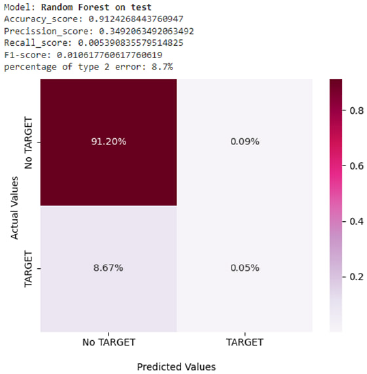
\includegraphics[width=\textwidth]{assets/121}
			\caption*{\bfseries Рис. 3 - Результаты случайного леса}
		\end{subfigure}
		\hfill
		\begin{subfigure}[b]{0.45\textwidth}
			\centering
			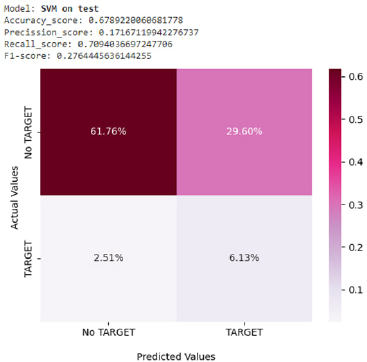
\includegraphics[width=\textwidth]{assets/122}
			\caption*{\bfseries Рис. 4 - Результаты машины опорных векторов (SVM)}
		\end{subfigure}
		
	\end{figure}
\begin{multicols}{2}
Результаты случайного леса (Random Forest): точность - хорошая, но
увеличилось и количество ошибок второго рода. Эта модель редко
предсказывает, что человек не вернет кредит.

Результаты SVM: эта модель показывает средние результаты при сравнении
логистической регрессии и случайного леса.

Результат: из всех метрик лучше всего выделяется процент ошибок 2-го
типа, он достаточно мал, о чем свидетельствует показатель полноты.
Точность приемлемая.

\end{multicols}
\begin{figure}[H]
	\centering
	\begin{subfigure}[b]{0.45\textwidth}
		\centering
		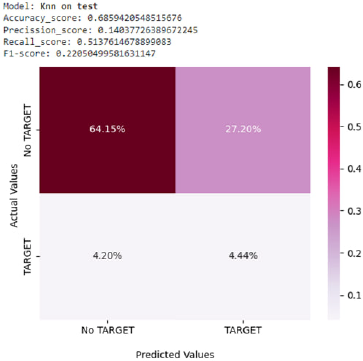
\includegraphics[width=\textwidth]{assets/123}
		\caption*{\bfseries Рис. 5- Результаты $k$ ближайщих соседей (KNN)}
	\end{subfigure}
	\hfill
	\begin{subfigure}[b]{0.45\textwidth}
		\centering
		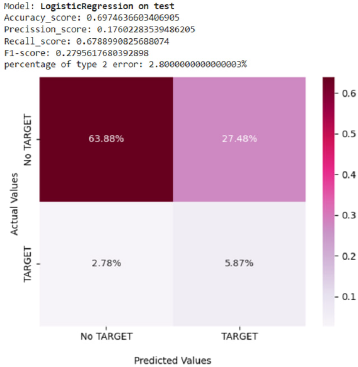
\includegraphics[width=\textwidth]{assets/124}
		\caption*{\bfseries Рис. 6 - Результаты логистической регрессии (LR)}
	\end{subfigure}
	
\end{figure}

\begin{table}[H]
    \caption*{Таблица 2 -- Результаты использованных моделей}
    \centering
    \begin{tabularx}{\textwidth}{|>{\centering\arraybackslash}X|>{\centering\arraybackslash}X|>{\centering\arraybackslash}X|>{\centering\arraybackslash}X|>{\centering\arraybackslash}X|}
    \hline
    Модели                        & Accuracy & Precision & Recall & F1-score \\ \hline
    Случайный лес (Random Forest) & 0.91     & 0.35      & 0.006  & 0.01     \\ \hline
    Машины опорных векторов (SVM) & 0.68     & 0.17      & 0.71   & 0.28     \\ \hline
    \emph{k}-Ближайших соседей (KNN)      & 0.69     & 0.14      & 0.51   & 0.22     \\ \hline
    Логистическая регрессия       & 0.70     & 0.18      & 0.68   & 0.28     \\ \hline
    \end{tabularx}
\end{table}


\begin{multicols}{2}

{\bfseries Выводы.} В статье проведено исследование кредитного скоринга с
использованием различных машинных алгоритмов. Основной целью
исследования было создание эффективной скоринговой модели для
прогнозирования вероятности дефолта клиентов Хоум Кредит Банка. Для
достижения этой цели был использован обширный набор данных,
предоставленный Хоум Кредит Банком, содержащий информацию о клиентах и
\hspace{0pt}\hspace{0pt}их кредитной истории. Данные были предварительно
обработаны и прошли этапы очистки, масштабирования и преобразования для
подготовки к обучению модели. В исследовании применялись четыре
различных моделей машинного обучения: случайный лес, машины опорных
векторов (SVM), $K$ ближайших соседей
(KNN), логистическая регрессия. Каждая модель была обучена на обучающей
выборке и протестирована на тестовой выборке. Эксперименты позволили нам
сравнить производительность различных моделей и оценить их точность,
полноту и F1-меру на основе показателей качества классификации.
Результаты показали, что модели Random Forest, Gradient и логистической
регрессии демонстрируют наилучшую точность и полноту. Они достигают
высокой точности прогнозирования кредитного риска и принимают
эффективные решения на основе предоставлен-ных данных. По результатам
экспериментов можно сделать следующие выводы: Модель, основанная на
ансамблевых методах, такой как Random Forest, показала лучшую
производительность среди всех протестированных моделей. Она
продемонстрировала высокую точность и стабильность в прогнозировании
кредитоспособности клиентов. Линейная модель, как логистическая
регрессия, показала низкую производительность по сравнению с другими
моделями. SVM также показала хороший результат, но немного уступали
ансамблевым моделям в точности прогнозирова-ния. KNN оказалась наименее
эффективнымм моделям среди протестированных. Они имеют ограниченные
возможности по моделированию сложных зависимостей в данных и требуют
более тщательного подбора параметров для достижения высоких результатов.
Оценка выполнения задачи показала, что использование Random Forest
позволяет существенно повысить точность прогнозирования
кредитоспособности клиентов. Эта модель обладают способностью обобщать
данные и фиксировать сложные взаимосвязи между атрибутами, что
обеспечивает высокую точность. Пути реализации результатов исследования
могут включать следующие аспекты: финансовым организациям рекоменду-ется
интегрировать выбранные ансамблевые модели, такие как Random Forest,
KNN, SVM LightGBM в свою систему кредитного скоринга. Это поможет
повысить качество и достоверность прогноза погашения кредита и снизить
риск для банка.

\end{multicols}

\begin{center}
{\bfseries Литература}
\end{center}

\begin{noparindent}

1.G.T.Balakayeva, D.K.Darkenbayev, C.Phillips. Investigation of
technologies of processing of BigData//\\International Journal of
Mathematics and Physics-2017.-Vol.8.- No.2.- P. 13-18. DOI:~10.26577/\\ijmph.2017.v8.i2.02

2.Anderson R. The credit scoring toolkit: theory and practice for retail
credit risk management and decision automation, N.Y.: Oxford University
Press, 2007. -- 790 p. ISBN: 9780199226405

3.Lewis E.M. An introduction to credit scoring.//Athena press, 1992. --
162 p.

4.Naeem S. Credit risk scorecards: developing and implementing
intelligent credit scoring//John Wiley and Sonsю- 2015.-208 p. ISBN:
978-1-119-20173-1

5.Allison P.D. Logistic regression using the SAS system: theory and
application//Cary, NC: SAS Institute, 2001. -- 303 p. SBN:
978-0-471-22175-3

6.Mays E.(ed.) Handbook of credit scoring. Chicago: Glenlake Publishing
Company Ltd /Fitzroy Dearborn Publishers, 2001.-370 p. ISBN
978-0814406199

7.Rimmer J. Contemporary changes in credit scoring // Credit Control,
2005.-Vol.4(26)- P.56-60.

8.Rowland J. B. Confidently evaluate small businesses with credit
scoring // Business Credit, 2003.- P. 26-31.

9.G. Balakayeva, D. Darkenbayev. The solution to the problem of
processing Big Data using the example of assessing the solvency of
borrowers//Journal of Theoretical and Applied Information Technology,
2020. -- Vol. 98(3).- P 2659-2670.

10.D. Darkenbayev Big Data processing on the example of credit
scoring,//Journal of Problems in Computer Science and Information
Technologies.-2023. -Vol.1(3).- P.50-61. DOI 10.26577/1i32jpcsit2307

11.Thomas Lyn C. A survey of credit and behavioural scoring: forecasting
financial risk of lending to consumers // International Journal of
Forecasting, 2000. -- No.16. -- Pp. 149-172.

12.Myers J.H., Forgy E.W. The development of numerical credit evaluation
systems//Journal of American Statistical
Association.-1963.-No.58.-P.799-806.

13. David W. Hosmer,~Stanley Lemeshow Applied logistic regression. -
N.-Y.: John Wiley and Sons, 2000. - P.1162-1163. DOI:10.1002/0471722146
\end{noparindent}

\begin{noparindent}

\emph{{\bfseries Сведения об авторах}}

Даркенбаев Д.К. - PhD, и.о. доцента, Казахский национальный университет
им. аль-Фараби, Алматы, Казахстан, e-mail: dauren.kadyrovich@gmail.com;

Зиятбекова Г.З.- PhD, и.о. доцента, Казахский национальный университет
им. аль-Фараби, Алматы, Казахстан, e-mail: ziyatbekova@mail.ru;

Алтыбай А. - PhD, и.о. доцента, Казахский национальный университет им.
аль-Фараби, Алматы, Казахстан,e-mail: arshyn.altybay@gmail.com;

Мекебаев Н.О.-PhD, ассоциированный профессор, Казахский национальный
женский педагогичес-кий университет, Алматы, Казахстан, e-mail:
nurbapa@mail.ru

Жамангарин Д. С.- PhD, Казахский университет технологии и бизнеса имени
К. Кулажанова, Астана, Казахстан, е-mail: Dus\_man89@mail.ru
\end{noparindent}



\emph{{\bfseries Information about the authors}}

\begin{noparindent}

Dauren D.-PhD, Acting Associate Professor Al-Farabi Kazakh National
University, Almaty, Kazakhstan, 
\\e-mail: dauren.kadyrovich@gmail.com;

Ziyatbekova G{\bfseries .-} PhD, Acting Associate Professor Al-Farabi
Kazakh National University, Almaty,\\ Kazakhstan,
e-mail:ziyatbekova@mail.ru;

Altybay A.-PhD, Acting Associate Professor Al-Farabi Kazakh National
University, Almaty, Kazakhstan,e-mail: arshyn.altybay@gmail.com;

Nurbapa M.-PhD, Associate Professor of the Department of Computer
Science, Kazakh National Women\textquotesingle s Pedagogical University,
Almaty, Kazakhstan,e-mail: nurbapa@mail.ru

Zhamangarin D. S.-PhD, K. Kulazhanov Kazakh University of Technology and
Business, Astana, \\Kazakhstan,е-mail: Dus\_man89@mail.ru.
\end{noparindent}
